\documentclass[a4paper, 12pt]{article}
\usepackage{a4wide}
\usepackage{graphicx}
\usepackage{xcolor}
\usepackage{hyperref}
\usepackage{wrapfig}
\renewcommand{\familydefault}{\sfdefault} % Use default sans-serif font

\usepackage{listings}

\usepackage[english]{babel}
\usepackage[latin1]{inputenc}

\lstloadlanguages{Lisp}

\lstset{
  basicstyle=\ttfamily\small,
  % numbers=left,numbersep=5pt,stepnumber=5,
  language=Lisp,
  backgroundcolor=\color{brown!20},
  keywordstyle=[1]{\ttfamily\color{blue}},
  keywordstyle=[2]{\itshape\color{blue}},
  morekeywords=[1]{handler-bind,with-open-file,while,with-sequence-residues},
  morekeywords=[2]{lambda},
  deletekeywords={collect,identity,length,list,mapcar,member,subseq},
  commentstyle=\color{red!90!green!90!blue},
  stringstyle=\color{brown},
  showstringspaces=false,
  captionpos=b}

\begin{document}

\title{cl-genomic : A Common Lisp library for processing genomic
  sequence data}
\author{Keith James}
\date{\today}

\maketitle

\section{Introduction}
\label{sec:intro}

cl-genomic is a portable Common Lisp library for processing genomic
data, including DNA, RNA and amino-acid sequences, and the biological
relationships between them.

\subsection{Design goals}
\label{sec:design}

\subsubsection{Uniform representation of  sequence and annotation}
\label{sec:seqrep}

The ``sequence feature'' is a common bioinformatics meme, often
represented in object-oriented programming by its own class hierarchy
that exists in parallel to the sequence class hierarchy. However, the
biological entities that these features represent are essentially
sequences. cl-genomic avoids use of the ``sequence feature'' as a
non-sequence type, substituting for them ``intervals'' that are
first-class sequences.

\subsubsection{Support for formalised biological concepts}
\label{sec:biorel}

A key goal for cl-genomic is support for formal representation of
biological concepts and their relationships. While cl-genomic may be
used without an ontology, the aim is to use the Sequence Ontology for
all non-trivial cases. In doing so, it is important to avoid
hard-coding biological knowledge into the API. For example, functions
such as \lstinline!transcript-of! or \lstinline!exon-of! are avoided
because they are only relvant and correct for a subset of biological
use cases. Instead, functions have ontology term parameters to convey
this information, when required.

The best choice of third-party ontology management and reasoning
software to use with cl-genomic is an open question. Candidates
include PowerLoom, various OWL and RDF stores (with a plethora of
incompatible and immature query languages), several SQL-based
bio-ontology warehouses and Prolog. The field is very fragmented and
the technology is not quite there yet.


\subsubsection{Support for whole genomes and short-read sequence data}

Good performance is required for datasets ranging from whole eukaryote
chromosomes to the hundreds of millions of short sequencing reads
produced per experiment by newer DNA sequencing technologies.


\subsubsection{Limited support for bioinformatics file formats}
\label{sec:bioformats}

cl-genomic will only support bioinformatics file formats that fall
into one or more of the following categories:

\begin{itemize}
\item Are structurally and semantically well-defined
\item Are simple enough to be trivial
\item Are so ubiqitous that they cannot be avoided
\end{itemize}

There exist other toolkits (notably BioPerl) that will read and write
many formats. Supporting file formats that have been used beyond the
original designers' intent, or were poorly designed in the first
place, is a significant burden. cl-genomic does not intend to
replicate that effort.

\subsection{Alternatives}
\label{sec:alternate}

The \href{http://common-lisp.net/project/cl-bio}{cl-bio} project.
\href{http://www.biolisp.org}{BioBike}.


\section{Creating bio-sequences}
\label{sec:makinging-bioseq}

\subsection{Making sequences from strings}
\label{sec:make-bioseq-str}

There exist three exported functions that create sequence objects from
strings; \lstinline!make-dna!, \lstinline!make-rna! and
\lstinline!make-aa!, creating DNA, RNA and amino-acid sequence objects
respectively.

Unless an \lstinline!:identifer! keyword argument is supplied, the
resulting object will be an anonymous sequence (i.e. will have an
identifier NIL and will return T if passed to the
\lstinline!anonymousp! predicate). A newly created nucleic-acid
sequence object will be double-stranded unless a
\lstinline!:num-strands! argument of 1 is supplied. The strandedness
of a sequence affects some operations. For example, it is not possible
to request an interval from the reverse-complement strand of a such a
sequence.

\begin{lstlisting}[caption={Making DNA sequences from strings},
  label=lst:make-dnaseq-string,float=[tbph]]
  (in-package :bio-sequence)
  
  ;; Create an anonymous DNA sequence
  (make-dna "gtaaaacgacggccagtg")
  
  ;; Use of characters illegal in DNA will cause an error
  (make-dna "guaaaacgacggccagug")

  ;; Create an identified, single-stranded DNA sequence 
  (make-dna "gtaaaacgacggccagtg" :identity 'm13-fwd :num-strands 1)

  ;; Create a DNA sequence with ambiguities
  (make-dna "gtanarygacggccagtg")

  ;; Create a 30bp virtual DNA sequence
  (make-dna nil :length 30)
\end{lstlisting}

All sequences support the full IUPAC character set
\cite{PMID:2582368}. Alternatively, sequences may be created without
any explicit residues, supplying instead a \lstinline!:length!
initialization argument. The resulting object will be a virtual
sequence (i.e. will be composed implicitly of ambiguous residues and
will return T if passed to the \lstinline!virtualp!
predicate). Virtual sequences are useful for representing the relative
positions of sequence intervals where knowledge of the residues is not
required.

\subsection{Reading sequences from streams}
\label{sec:read-bioseq-stream}

Reading DNA, RNA or amino-acid sequences from a stream is essentially
a chunking operation; data such as sequence metadata and residue
characters are gathered until a complete sequence record has been
read, then the gathered data are processed in some way.

The generic function \lstinline!make-seq-input! is the entry point for
reading from streams. There are several methods available, all of
which accept two mandatory arguments; a stream designator (a string
naming a file, a pathname or a stream) and a format symbol. The
\lstinline!:alphabet! argument is used to specify the sequence
alphabet (\lstinline!:dna!, \lstinline!:rna! or \lstinline!:aa!,
defaulting to \lstinline!:dna!). Other keyword arguments are available
(see the API reference). The value returned is a generator function (a
closure, in fact) that may be passed to the general-purpose generator
API functions \lstinline!has-more-p! and \lstinline!next! to return
sequences.

The parsers offer restarts for occasions where badly formatted
sequence records are encountered, allowing such records to be skipped,
logged or otherwise handled using the standard CL (Common Lisp)
condition and restart system. The error conditions raised by the
parser will be \lstinline!general-parse-error!s, or a subtype thereof.

The basic restart function is \lstinline!skip-malformed-sequence!
which causes the generator to return NIL and moves the stream forward
to the next record.

\begin{lstlisting}[caption={Making sequences from streams},
  label=lst:read-bioseq-stream,float=[tbph]]
  (in-package :bio-sequence)
  
  ;; Read Fasta format DNA sequences from a named file into a list
  (with-open-file (stream "seq.fasta")
      (let ((seqi (make-seq-input stream :fasta)))
        (loop
           while (has-more-p seqi)
           collect (next seqi))))

  ;; Read a single AA sequence from a stream
  (next (make-seq-input stream :fasta :alphabet :aa))

  ;; Read the human genome in Fasta format from a file and print
  ;; chromosome names and lengths
  (with-open-file (stream "Homo_sapiens.NCBI36.52.dna.toplevel.fa")
      (let ((seqi (make-seq-input stream :fasta :virtual t)))
        (loop
           while (has-more-p seqi)
           do (let ((seq (next seqi)))
                (format t "~a ~a~%" (identity-of seq)
                        (length-of seq))))))

  ;; Read Fasta format DNA sequences, using restarts to skip
  ;; bad records
  (with-open-file (stream "bad_seq.fasta")
      (handler-bind ((malformed-record-error
                        #'skip-malformed-sequence))
        (let ((seqi (make-seq-input stream :fasta)))
           (loop
              while (has-more-p seqi)
              for seq = (next seqi)
              when seq
              collect seq))))
\end{lstlisting}

The parsing process may be customized by using the \lstinline!:parser!
argument of \lstinline!make-seq-input! to pass an instance of a
subclass of \lstinline!bio-sequence-parser!. For example, passing a
\lstinline!raw-sequence-parser!  will result in a generator that
returns assoc lists of sequence data instead of CLOS sequence objects.
This is useful in cases where performance is critical or wherethe
functionality provided by CLOS is unecessary. The parser protocol is
described in the API documentation.


\section{Memory-mapping bio-sequences from files}
\label{sec:memory-map-bioseq}

When using very large DNA sequences, such as entire eukaryotic
chromosomes, it may be more efficient to memory-map the data than to
read it from a stream. cl-genomic supports this mode of access by
means of mapped-dna-sequences. In addition, arbitrary memory-mapped
sequences may be created from automatically generated temporary
files. Macros are provided that automatically map and unmap the
sequence data safely.  To be memory-mapped, a sequence data file must
be in ``pure'' format, that is it must contain only ASCII tokens from
the correct alphabet and optionally a single terminating new- line
character. The \lstinline!convert-sequence-file! method provides a
means of preparing such files.



\begin{lstlisting}[caption={Memory-mapping a bio-sequence},
  label=lst:read-bioseq-stream,float=[tbph]]
  (in-package :bio-sequence)

  ;; Make a pure sequence file
  (convert-sequence-file "data/simple-dna1.fasta" :fasta
                         "data/simple-dna1.pure" :pure)

  ;; Memory map 100 bp of the sequence. Print its length and
  ;; make a list of its residues
  (with-mapped-dna (mseq :filespec "simple-dna1.pure" :length 100)
     (format t "len: ~a residues: ~a~%"
            (length-of mseq)
            (loop
               for i from 0 below (length-of mseq)
               collect (element-of mseq i))))

  ;; Create an anonymous, temporary 250,000,000 bp sequence of 'N's.
  ;; Return a 100 bp internal subsequence.
  (with-mapped-dna (mseq :length 250000000)
    (subsequence mseq 1000000 1000100))
\end{lstlisting}


\section{Bio-sequence alphabets}
\label{sec:alphabet-bioseq}

The permitted residues of DNA, RNA and amino-acid sequences are
represented by \lstinline!alphabet!s. Every \lstinline!bio-sequence!
instance contains its alphabet in a class-allocated slot, accessible
through the \lstinline!alphabet-of! reader. For reference, the list of
all available alphabets may be obtained by calling the
\lstinline!registered-alphabets! function, while individual alphabets
may be obtained by passing an alphabet name symbol (such as
\lstinline!:dna!, \lstinline!:rna! or \lstinline!:aa!) to the
\lstinline!find-alphabet! function. An alphabet object has several
slots, including its name and set of valid tokens, accessible via the
\lstinline!name-of! and \lstinline!tokens-of! readers, respectively.

An \lstinline!alphabet!'s set of tokens comprises all its unambiguous
and ambiguous tokens, plus a gap token. For example, the
\lstinline!:dna! alphabet contains characters for all of the IUPAC
codes (the \lstinline!:simple-dna! alphabet contains only 'a', 'c',
'g' and 't'). The \lstinline!size-of! method returns the size of an
alphabet which is defined as the number of tokens it contains. Higher
order alphabets may be constructed by using as tokens lists of
characters from other alphabets. In this way, the standard codon
alphabets are constructed.

To test whether a token is a member of an alphabet one can obtain the
alphabet's token list and use the standard CL \lstinline!member!
function, with an appropriate test predicate (the case of characters
is not significant). Alternatively, the \lstinline!memberp! method may
be used for convenience. Tokens that represent IUPAC ambiguity codes
may be analysed in the context their alphabets; they may be expanded
into equivalent lists of unambiguous tokens or tested to see whether
one subsumes the other i.e. that the unambiguous tokens represented by
one ambiguous token are a subset of those represented by another.

\begin{lstlisting}[caption={Using bio-sequence alphabets},
  label=lst:using-bioseq-alphabets,float=[tbph]]
  (in-package :bio-sequence)
  
  ;; List the names of the registered alphabets
  (mapcar #'name-of (registered-alphabets))

  ;; Make an assoc list mapping the alphabet names to their sizes
  (mapcar (lambda (x)
            (list (name-of x) (size-of x)))
          (registered-alphabets))

  ;; Is the character 't' in the DNA alphabet?
  (memberp #\t (find-alphabet :dna))

  ;; What characters does 'n' represent in the DNA alphabet?
  (enum-ambiguity #\n (find-alphabet :dna))

  ;; What unambiguous codons do 'nnn' represent in
  ;; the DNA codon alphabet?
  (enum-ambiguity '(#\n #\n #\n) (find-alphabet :dna-codons))

  ;; Does the character 'r' match the character 'n' in
  ;; the DNA alphabet?
  (subsumesp #\r #\n (find-alphabet :dna))

  ;; Does the codon 'aaa' match the codon 'raa' in
  ;; the DNA codon alphabet?
  (subsumesp '(#\a #\a #\a) '(#\r #\a #\a)
             (find-alphabet :dna-codons))
\end{lstlisting}


\section{Manipulating bio-sequences}
\label{sec:manipulating-bioseq}

\subsection{The components of a bio-sequence}
\label{sec:components-of-bioseq}

The simplest \lstinline!bio-sequence! objects contain little more than
slots for an identifier, an alphabet that describes the permitted
sequence residues and either a vector of residues or a length (in the
case of virtual sequences). While a description string slot is present
in all bio-sequence objects, it should be used with
care. \footnote{The description string is free text and therefore
  should only be used for round-tripping data between persistent
  storage. For example, it may be used to store the header line found
  in Fasta format files. It should not be computed upon.}  Nucleic
acid sequences also have a \lstinline!num-strands-of! method that may
be used to get and set the number of strands the sequence has.

The sequence residues themselves may be accessed through the
\lstinline!element-of! method (or its synonym
\lstinline!residue-of!). If the sequence has concrete residues (is not
virtual), the residues are \lstinline!setf!-able and thus may be
mutated. 

\begin{lstlisting}[caption={The components of a bio-sequence},
  label=lst:components-of-bioseq,float=[tbph]]
  (in-package :bio-sequence)

  ;; Create an anonymous DNA sequence. Print its identity, length
  ;; and make a list of its residues
  (let ((seq (make-dna "gtaaaacgacggccagtg")))
    (format t "id: ~a len: ~a residues: ~a~%"
            (identity-of seq) (length-of seq)
            (loop
               for i from 0 below (length-of seq)
               collect (element-of seq i))))

  ;; Create an anonymous DNA sequence and mutate all its residues
  ;; randomly
  (let ((seq (make-dna "gtaaaacgacggccagtg"))
        (dna (find-alphabet :simple-dna)))
    (loop
       for i from 0 below (length-of seq)
       do (setf (element-of seq i) (random-token-of dna))
       finally (return seq)))
  
  ;; Create an anonymous DNA sequence and mutate all its residues
  ;; randomly, this time using the with-sequence-residues macro
  (let ((seq (make-dna "gtaaaacgacggccagtg"))
        (dna (find-alphabet :simple-dna)))
    (with-sequence-residues (residue seq)
      (setf residue (random-token-of dna))))
\end{lstlisting}

The coordinate system used to address residues within a
\lstinline!bio-sequence! is a zero-based, inter-residue system
i.e. the boundaries between sequence residues are counted, starting
from zero. This is the same as the system used by the Chado genome
database \cite{gmod-chado} and equivalent to the zero-relative,
half-open residue-numbering system used by the UCSC genome database
\cite{PMID:18996895}. It is also the same as the indexing used by the
CL \lstinline!subseq! function, see Figure
\ref{fig:inter-residue-coords}. It would be rather inconvenient
to be required to use two inter-residue coordinates to address a
single residue, therefore an equivalent single-coordinate system is
provided; if a single inter-residue coordinate is provided, it
implicitly addresses the following residue. The resulting system is
equivalent to the standard addressing of CL vectors.

\begin{figure}[tbph]
  \begin{center}
    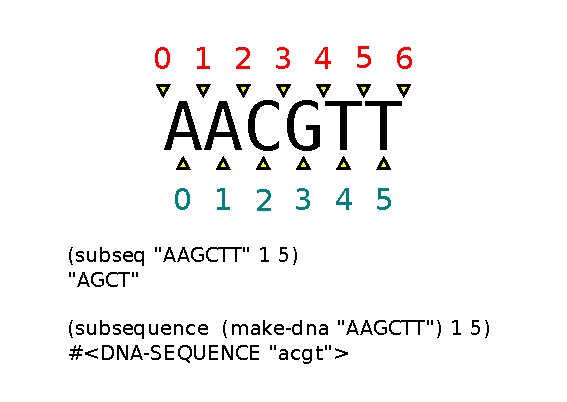
\includegraphics[scale=1.0]{inter-residue-coordinates.pdf}
  \end{center}
  \caption{The bio-sequence residue coordinate system. Explicit
    inter-residue coordinates are shown in red, equivalent implicit
    vector-style coordinates in blue.}
  \label{fig:inter-residue-coords}
\end{figure}

The strand of a nucleic acid sequence is represented by one of the
global strand objects \lstinline!*forward-strand*!,
\lstinline!*reverse-strand*! or \lstinline!*unknown-strand*!. There
exist a number of methods for testing, comparing and converting
strands. The convention for comparing two strands is that if either is
unknown, they cannot be \lstinline!strand=!. However, if both strands
are unknown they are \lstinline!strand-equal!. In other words, the
former test guarantees that the strands are the same, while the latter
guarantees only that they might be the same.

The complement relationship between forward and reverse strands is
executed by the \lstinline!complement-strand! method, while the
\lstinline!complementp! predicate tests for this relationship. The
complement of the unknown strand is itself the unknown strand. The
\lstinline!complementp! predicate is implemented using
\lstinline!strand=! and shares its restriction that it will return T
only if the strands are guaranteed to be complementary.

\begin{lstlisting}[caption={Sequence strand operations},
  label=lst:testing-bioseq,float=[tbph]]
  (in-package :bio-sequence)

  ;; Returns T
  (strand= *forward-strand* *forward-strand*)
  (strand= *reverse-strand* *reverse-strand*)

  ;; Returns NIL
  (strand= *unknown-strand* *unknown-strand*)
  
  ;; Returns T
  (strand-equal *forward-strand* *forward-strand*)
  (strand-equal *reverse-strand* *reverse-strand*)
  (strand-equal *unknown-strand* *unknown-strand*)
  (strand-equal *unknown-strand* *forward-strand*)
  (strand-equal *unknown-strand* *reverse-strand*)
  
  ;; Returns NIL
  (strand= *forward-strand* *reverse-strand*)
  
  ;; Returns T
  (complementp *forward-strand* *reverse-strand*)

  ;; Returns NIL
  (complementp *unknown-strand* *unknown-strand*)
  (complementp *forward-strand* *unknown-strand*)
  (complementp *reverse-strand* *unknown-strand*)
\end{lstlisting}


\subsection{Testing bio-sequences}

The various biological types of sequence are implemented as CLOS
classes, meaning that method dispatch may be used to select
appropriate code branches in many cases. The predicates testing
\lstinline!bio-sequence! ambiguity, strand count and virtual state
fall into this category, meaning that it is an error to use them on
non-\lstinline!bio-sequence! objects.

In addition, a set of predicates are provided for testing directly the
biological type of \lstinline!bio-sequence! objects. These are normal
functions and will simply return NIL if passed a Lisp object that is
not a \lstinline!bio-sequence!.

\begin{lstlisting}[caption={Testing bio-sequences},
  label=lst:testing-bioseq,float=[tbph]]
  (in-package :bio-sequence)

  ;; Create and test anonymous sequences
  (defparameter *example-dna*
       (list (make-dna "acgt" :num-strands 1) (make-dna "acgn")))
  (defparameter *example-rna*
       (list (make-rna "acgu") (make-rna "acgn")))
  (defparameter *example-aa*
       (list (make-aa "MAD") (make-aa "MAB")))
  (defparameter *example-seq*
       (concatenate 'list *example-dna* *example-rna*
                    *example-aa*))

  ;; Generic function methods
  (mapcar #'simplep *example-seq*)
  (mapcar #'ambiguousp *example-seq*)
  (mapcar #'virtualp *example-seq*)
  
  (mapcar #'single-stranded-p *example-dna*)
  (mapcar #'double-stranded-p *example-rna*)

  ;; Returns T if all sequences have the same number of strands
  (apply #'same-strand-num-p *example-dna*)
  (apply #'same-strand-num-p *example-rna*)
  
  ;; Functions
  (mapcar #'bio-sequence-p *example-seq*)
  (mapcar #'dna-sequence-p *example-seq*)
  (mapcar #'rna-sequence-p *example-seq*)
  (mapcar #'aa-sequence-p *example-seq*)

  ;; Returns T if all sequences have the same biological type,
  ;; DNA, RNA or AA
  (apply #'same-biotype-p *example-dna*)
  (apply #'same-biotype-p *example-seq*)
\end{lstlisting}

\subsection{Coercing bio-sequences}
\label{sec:coerce-bioseq}

In the same way that CL types may be coerced, it is possible to coerce
\lstinline!bio-sequence! s, either to other \lstinline!bio-sequence!
types or to CL strings. In fact, coercion to a string is the main way
of producing a bare string rendering of a
\lstinline!bio-sequence!. Bio-sequence coercion differs from CL
coercion in that the function accepts \lstinline!:start! and
\lstinline!:end! arguments, making it possible to coerce a subsequence
directly, without first using the \lstinline!subsequence! method.

\begin{lstlisting}[caption={Coercing bio-sequences},
  label=lst:coercing-bioseq,float=[tbph]]
  (in-package :bio-sequence)

  ;; DNA may be coerced to RNA and vice versa
  (coerce-sequence (make-dna "acgt") 'rna-sequence
  (coerce-sequence (make-rna "acgu") 'dna-sequence)

  ;; A virtual sequence may be coerced to a concrete sequence
  (coerce-sequence (make-dna nil :length 4) 'dna-sequence)

  ;; Sequences may be coerced to strings
  (coerce-sequence (make-dna "acgt") 'string)
  (coerce-sequence (make-dna "acgt") 'string :start 0 :end 2)
  (coerce-sequence (make-aa "MAD") 'string)
\end{lstlisting}


\bibliographystyle{plain}
\bibliography{cl-genomic}

\end{document}
